% Created 2025-09-10 Wed 23:46
% Intended LaTeX compiler: pdflatex
\documentclass[compress,dvipdfmx,11pt]{beamer}
\usepackage[utf8]{inputenc}
\usepackage[T1]{fontenc}
\usepackage{graphicx}
\usepackage{longtable}
\usepackage{wrapfig}
\usepackage{rotating}
\usepackage[normalem]{ulem}
\usepackage{amsmath}
\usepackage{amssymb}
\usepackage{capt-of}
\usepackage{hyperref}
% \title[2025 年度 電子情報通信学会 ソサイエティ大会]{\bf 未知のグラフにおけるレジリエンス向上のためのアンカーノード探索手法に関する一検討}
% \institute{関西学院大学 工学部 情報工学課程 $^1$  \\ 関西学院大学 大学院理工学研究科 情報科学専攻 $^2$}
% \date{2025 年 9 月 11 日}
% \setlength{\parskip}{1.5ex}
% \renewcommand{\textbf}{\alert}
% \usetheme{Ohsaki}
% \author{石本 哲郎 \(^1\) 井上 翔太 \(^2\) 大崎 博之 \(^2\)}
% \date{2025 年 9 月 11 日}
% \begin{document}

\title[中間審査]{\bf  未知のグラフにおけるレジリエンス向上のためのアンカーノード探索手法に関する一検討}
\author[]{石本 哲郎}
\institute{関西学院大学 工学部 情報工学課程}
\date{2025 年 9 月 18 日}
\setlength{\parskip}{1.5ex}
\renewcommand{\textbf}{\alert}
\usetheme{Ohsaki}
\begin{document}



\maketitle
\begin{frame}{Outline}
\tableofcontents
\end{frame}

\newcommand{\pivec}{\mathbf \pi}
\newcommand{\xvec}{\mathbf x}
\newcommand{\yvec}{\mathbf y}
\newcommand{\zvec}{\mathbf z}
\newcommand{\Emat}{\mathbf E}
\newcommand{\Imat}{\mathbf I}

\bf
\section{はじめに}
\label{sec:org8d9d03d}
\begin{frame}[label={sec:org3682d4b}]{研究の背景 : ネットワークレジリエンスの必要性}
\begin{itemize}
\item 現代社会と通信ネットワーク
\begin{itemize}
\item 高度情報化社会において、通信ネットワークや社会基盤システムは不可欠
\item 生活・経済・産業・医療など、あらゆる活動が依存している
\item 災害・故障・サイバー攻撃などのリスクに備える必要がある
\end{itemize}
\end{itemize}

\vspace{3mm}

\alert{レジリエンスを確保することは極めて重要な課題}
\begin{itemize}
\item レジリエンス:障害や攻撃を受けても、機能を維持し続けられる能力
\end{itemize}
\end{frame}
\begin{frame}[label={sec:org97a22d9}]{研究の動機 : 先行研究と課題}
\begin{itemize}
\item 既存のレジリエンス向上のアプローチ
\begin{itemize}
\item 障害や攻撃を受けても機能を維持するためにはどのノードを保護すれば良いかを考える
\item 既存研究では、限られたコストでレジリエンス向上に最も寄与するノード
を逐次的に選択する貪欲アルゴリズム AdvGreedy が提案された
\end{itemize}

\item しかしながら、ネットワーク全体のトポロジカルな構造が完全に既知であり、
任意のノードの状態を即座に把握できるという仮定に基づく
\end{itemize}

\vspace{2mm}

→ 未知のネットワーク上では利用できない
\end{frame}
\begin{frame}[label={sec:orgb9b5a98}]{研究の目的}
\begin{itemize}
\item 本研究の想定
\begin{itemize}
\item ネットワーク全体の構造は未知
\item 未知のネットワークを \alert{ランダムウォーク} により探索
\begin{itemize}
\item グラフの頂点を確率的に遷移していくプロセス
\item 訪問したノードを「探索済み」として記録
\end{itemize}
\item ランダムウォークで得られる \alert{部分的な情報} のみが利用可能
\end{itemize}
\end{itemize}

\vspace{3mm}

\begin{itemize}
\item 本研究の目的
\begin{itemize}
\item このような条件で、不完全情報下におけるアンカー選定戦略の有効性を明らかにする
\end{itemize}
\end{itemize}
\end{frame}
\section{RW によるアンカーノード探索}
\label{sec:org0282284}
\begin{frame}[label={sec:orgd25499c}]{フォロワー最大化問題 (1/2)}
\begin{itemize}
\item 先行研究では、レジリエンス向上をフォロワー最大化問題として定式化することで解いている
\end{itemize}

フォロワー最大化問題の概要
\begin{itemize}
\item レジリエンス利得を最大化するアンカーノードの組合せを求める
\begin{itemize}
\item レジリエンス利得 : 保護されるノードの総数
\item ノードの保護 : あるノードから少なくとも一つのアンカーノードに対し
て、障害のない安定した経路上で到達可能であること
\item アンカーノード : 障害を受けない特別なノード
\end{itemize}
\end{itemize}

どのようにアンカーノードを設定すれば、最大のフォロワーを得られるかを解く
\end{frame}
\begin{frame}[label={sec:orged383bc}]{フォロワー最大化問題 (2/2)}
フォロワー最大化問題の定義
\begin{itemize}
\item 入力
\begin{itemize}
\item 無向グラフ \(G\)
\item アンカー設置の総予算 \(b\)
\end{itemize}

\item 出力
\begin{itemize}
\item アンカーの集合 \(A\)
\end{itemize}

\item 制約条件
\begin{itemize}
\item 設定したアンカーノードの数が予算内であること : \(|A| \leq b\)
\end{itemize}

\item 目的
\begin{itemize}
\item 保護されるノードの数を最大化する
\end{itemize}
\end{itemize}
\end{frame}
\begin{frame}[label={sec:org27a6bc8}]{ランダムウォークによるアンカーノード探索の概要}
\begin{itemize}
\item 未知グラフでのアンカーノード探索を行なうアイデア
\begin{itemize}
\item ランダムウォークによってグラフを探索する
\item ランダムウォークで探索した部分グラフを入力として、フォロワー最大化問題を解く
\item その際のフォロワー最大化問題は既存の手法を用いて解く
\end{itemize}
\end{itemize}
\end{frame}
\begin{frame}[label={sec:orgf33e666}]{ランダムウォークによるアンカーノード探索}
\begin{itemize}
\item 具体的なアンカーノード選定方法
\begin{enumerate}
\item 探査エージェントがランダムウォークを開始する
\item 探索エージェントが訪問したノード、リンクを記録する
\item ある探査ステップ \(k\) 経過後、記録したノードとリンクから構築されたグラフ \(G'(k)\) を取得する
\item 既存手法で提案されたアンカーノード決定手法 AdvGreedy を \(G'(k)\) に適用する
\item グラフ \(G'(k)\) におけるアンカーノードの集合 \(A_k\) を得る
\end{enumerate}
\end{itemize}
\end{frame}
\section{実験}
\label{sec:org7e13e3d}
\begin{frame}[label={sec:org03810a4}]{実験の目的と設定}
\begin{itemize}
\item 実験の目的
\begin{itemize}
\item ランダムウォークによるアンカーノード探索の有効性を検証する
\end{itemize}

\item 実験の設定
\begin{itemize}
\item グラフの種類 : ランダムグラフ、BAグラフ
\item 使用したランダムウォーク戦略 : SRW,NBRW,VARW,SARW
\item ランダムウォークの開始地点 : 10個
\item ランダムウォークの試行回数 : 100回
\item ステップ数 : 0から300
\end{itemize}

\item 評価指標
\begin{itemize}
\item シミュレーション結果のフォロワー数とネットワーク全体を入力値としたときのフォロワー数の比較
\item ネットワーク全体を入力としたときのネットワークレジリエンスはそれぞれランダムグラフでは15、BAグラフでは30であった
\end{itemize}
\end{itemize}
\end{frame}
\begin{frame}[label={sec:org8e277fb}]{結果}
\begin{center}
\begin{figure}[h!]
  \begin{minipage}[t]{0.45\textwidth}
    \centering
    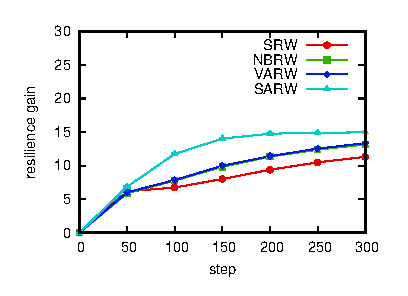
\includegraphics[width=\textwidth]{./figure/random-result.eps}
    \caption{ランダムグラフの結果}
  \end{minipage}
  \hfill
  \begin{minipage}[t]{0.45\textwidth}
    \centering
    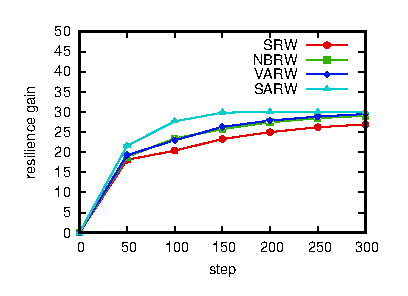
\includegraphics[width=\textwidth]{./figure/ba-result.eps}
    \caption{BAグラフの結果}
  \end{minipage}
\end{figure}
\end{center}
\begin{itemize}
\item ランダムグラフにおいてもBAグラフにおいてもSARWが最も高いレジリエンスゲインを早期に達成できる
\end{itemize}
\end{frame}
\section{まとめ}
\label{sec:org4b3d7d5}
\begin{frame}[label={sec:orgeadf93c}]{まとめと今後の課題}
\begin{itemize}
\item まとめ
\begin{itemize}
\item 既知ネットワークにおけるフォロワー最大化問題を未知ネットワークに適用
\item 未知ネットワークに対して高いレジリエンスゲインを早期に発見できるランダムウォーク戦略を検証
\end{itemize}

\item 今後の課題
\begin{itemize}
\item 他のトポロジ構造の場合では探索手法ごとにどのような変化があるかを検証する
\item より大規模なグラフに対しても有効性を検証する
\end{itemize}
\end{itemize}
\end{frame}
\end{document}
